
\section{Method}

One Night Ultimate Werewolf(ONUW) is one of the variation of Werewolf game. Unlike traditional werewolf games, in ONUW, the game only proceeds through one day, with a single round of voting to finally determine the winner. Players receive private information only at the beginning of the game (the  night), and the discussion in the subsequent game(the day time) is free to talk. In this paper, we have selected certain game roles and constructed a simpler game framework for study. Specific game rules and the framework are detailed in Appendix \ref{sec:Appendix_ONUW_game}.

\subsection{Humanized Agent}

\begin{figure*}[ht]
  \centering
  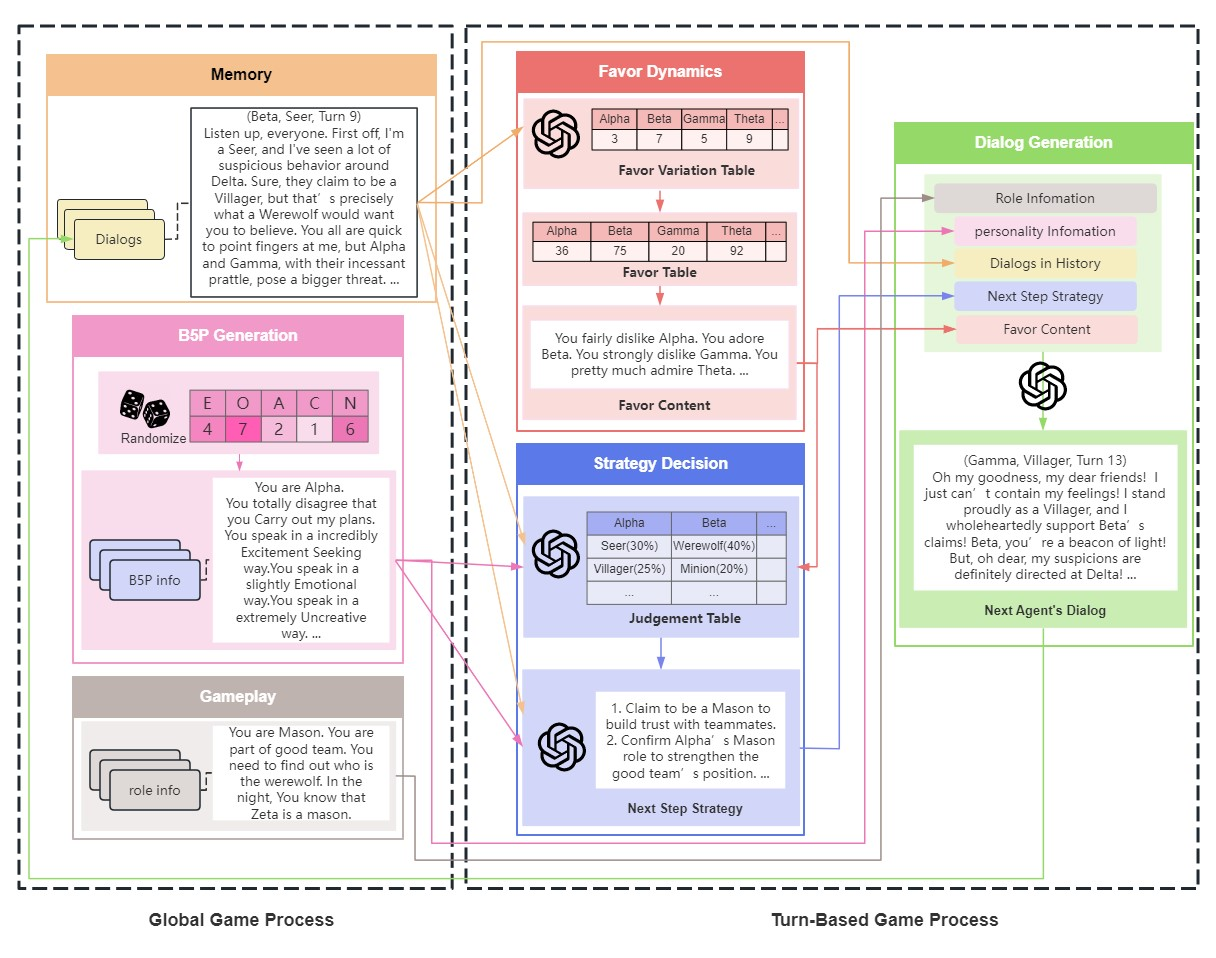
\includegraphics[width=0.99\textwidth]{img/framework.jpg}
  \caption{ Overview of Humanized Agent architecture. (1) Game History: a memory pool of what agents do and say in the game. (2) B5P Generation: a process to generate randomized Big Five Personality descritpion for each agnent. (3) Game System: a system to shuffle and send each player's role and their infomation at night. (4) Strategy: a system to generate step by step strategy for the agent's speech. (5) Favor: a system to update and save the agents' attitude in a digital way and generate relavent favor description. (6) Dialog: a process for collecting pregenerated data and generating the final talk }
\label{fig:framework}
    \vspace{-1em}
\end{figure*}

Humanized Agent aim to provide a framework for generating dialogue behavior in non-complete-information social games: they can self-guide their strategies based on system rules and information generated by other agents, and they possess individual conversational tastes and distinct attitudes. The design of such agents aims to replicate the strategies human players might employ during gameplay, ensuring the generated game content remains coherent. Additionally, the framework increases the diversity and excitement of the gameplay, as player strategies change due to personality and favorability, leading to varied game flows. The content generated by large language models inherently possesses a certain degree of randomness, which may not only allow our system to enable the agent to produce variations across multiple game sessions in response to changes in the game's progression, but also help maintain the overall logical consistency and coherence of the game.

In our framework, we incorporate the Big Five Factor theory from psychology to randomly define the underlying traits of the agents and introduce the concept of "favorability" to describe the degree to which an agent likes the speech of other agents. Inspired by the Chain of Thought approach \citep{wei2022chain}, we implement a strategy decision system to enhance the richness and rationality of the agent's decision-making. Moreover, drawing from the experience of generative agents in memory storage \citep{park2023generative}, we optimize how agents select and organize historical information. In summary, we innovatively propose an affective agent system to meet the needs for rich and coherent conversation content in social game conversation generation. Our system can be broken down into several subsystems: the B5P Generation System, the Strategy Decision System, the Favor System, Dialog Generation System and two supporting systems, including Gameplay System and Memory System.


Figure~\ref{fig:framework} illustrates the overall framework of our agent system. Firstly, the B5P Generation System, which is used to create personality traits for each participating agent, and the Gameplay System, which randomly assigns roles to each agent and disseminates relevant game information to them, are executed in the begining of the game to generate globally usable information.  Secondly, the Memory System serves as the storage for the agents' memory, storing chats in a list format and ranking the importance of each conversation, retrieving the top K conversations for use. Then, the Favor Dynamics System, the Strategy Decision System, and the Dialog Generation System are systems called before each agent speaks during the game. The Favor Dynamics System makes one LLM request to evaluate each other agent and updates the favorability ratings based on the results. On the other hand, two LLM requests are made by the Strategy Decision System  to determine the next strategic move in the game. The Dialog Generation System synthesizes the information obtained from the aforementioned systems to generate the agents' conversations for the current turn.


\subsection{Big Five Persona(B5P) Generation} \label{sec:B5P_System}

\begin{figure*}[ht]
  \centering
  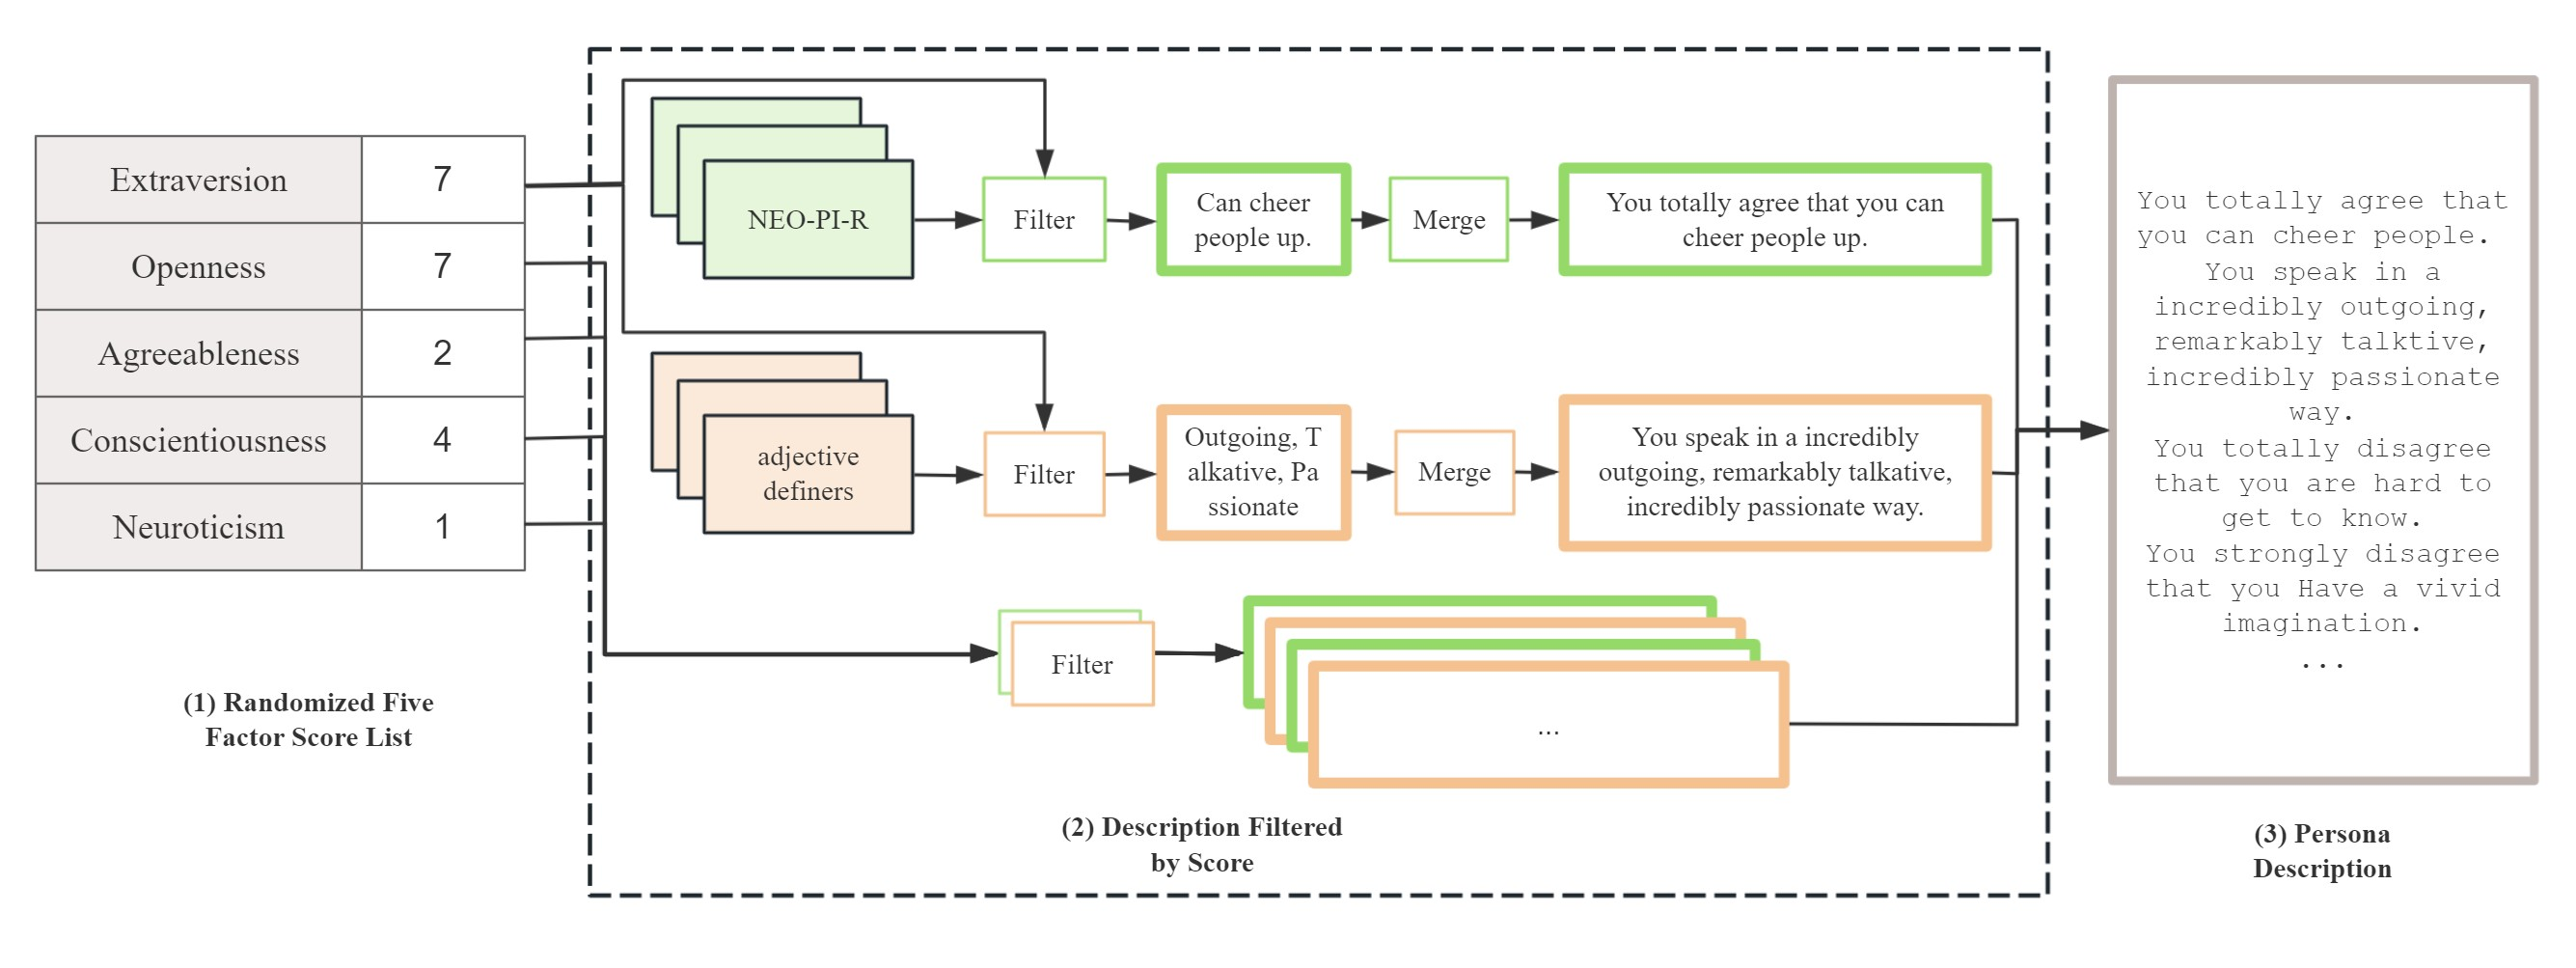
\includegraphics[width=0.99\textwidth]{img/B5P_framework2.jpg}
  \caption{ The framework of how to generate B5P statement.  (1) Randomized Big Five factor Score Set: a set of five random number range from 1-7, representing the five factor in FFM. (2) Description Filtered by Score: Select the statements from NEO-PI-R and adjective definders and combine them in a readable way according to the score list (3) B5P Statement: combine all five factors' descritpion together and form a final B5P statement. }
\label{fig:B5P_framework}
    \vspace{-1em}
\end{figure*}


\textit{Issue} For the same or similar question descriptions, LLMs, due to their pursuit of accuracy, tend to provide answers with similar meaning and phrasing. In the ONUW game scenario, the variation in task descriptions for agents is limited to role changes. Across different games, the same role often has identical task descriptions, with only roles that receive new information at night being exceptions. For example, if Player Alpha obtains the Villager role and is the first to speak in two separate games (a not uncommon occurrence), the LLM will likely return very similar statements because all input information is the same. Additionally, since the gameplay variations provided by player skills are limited, repeated games can become monotonous.

\paragraph{Method} In out method, the B5P description is introduced to provide diversity in agent expression and decision-making. Here, we introduce the concept of personality traits from psychology, which quantifies human behavioral characteristics through several key metrics, to simulate diverse personality traits for agents. We adopt the Big Five Personality theory's Five Factor Model to quantitatively simulate the personality traits of agents. For each agent participating in the game, we generate and assign a random personality profile that remains consistent throughout the game. Before each LLM query, we describe the agent according to this profile, thereby shaping the agent to embody the specific personality traits.

We first quantify the five factors of the Big Five Personality model: Extraversion, Openness, Agreeableness, Conscientiousness, and Neuroticism, using a scale from 1 to 7, where 1 represents a weak manifestation of the trait and 7 a strong one. From the NEO-PI-R, we can find positive and negative statements for each factor. We extract these statments and augment them with adverbs indicating the degree of agreement, such as 'totally agree,' 'slightly disagree,' etc., to create quantified evaluations for the different factors. Adjective descriptions for the various factors, summarized by Costa and McCrae, have also been carefully collected and organized into a factor-adjective dictionary. We use the pattern "You speak in a [adjective] way" to constrain the linguistic behavior of the agents, which has proven to be the most effective among the various descriptive approaches we've tried. Through multiple experiments, we found that when the trait value is closer to moderate, i.e., around 4, the description of that trait becomes less distinct. Conversely, when the trait value is closer to the extremes, such as 1 or 7, the description becomes more pronounced, and the agent exhibits a stronger personality. Therefore, in our framework, we use a random function to select which traits are described more frequently—the closer a trait value is to 1 or 7, the more likely it is to be described. The framework of our method is shown in Figure~\ref{fig:B5P_framework}

We suppose the agents are numbered by $ i $. Each agent has a persona represented by a list of big five factor scores $ B_i $. The five factor is represented by a score $ b_k $, in the range of 1 to 7, where $ k $ means the index of factor. Then we can have:
\begin{equation}
  B_i ={\left\{ b_k \right\}}_{k=1}^{5}
\end{equation}

In the process of descritpion generation, we turn the set of five factor scores into a piece of persona descriptions. We define the function $ F_D(b_k) $ to determine the degree statement according to the factor score $ b_k $. Firstly, the statements from NEO-PI-R are extracted based on th the factor $ k $ through $ F_N(k) $. While the adjective definition is generated from $ F_A(k) $. Both $ F_N(k) $ and $ F_A(k) $ will randomly select one descritpion from the dataset. We will define a resampled counter function $ F_R(b_k) $ to determine the number of times different factor scores will be resampled. The closer a factor score is to 1 or 7, indicating that the factor is more pronounced, the higher the number of resamples returned by the sampling function will be. Finally, we use a merge function $ F_M(n, a, r, f) $, which can complete the descritpion content according to the factor score $ b_k $, to obtain the final B5P statement. Here we have:
\begin{equation}
  F_D(b_k) = F_M( {\left\{ F_N(k), F_A(k) \right\}}_{t=1}^{F_R(b_k)}, b_k)
\end{equation}
So for each agent, we are able to produce the B5P statement $ \mathcal{B}_i $:
\begin{equation}
   F_D(B_i) = \bigcup_{k=1}^{5} F_M( {\left\{ F_N(k), F_A(k) \right\}}_{t=1}^{F_R(b_k)}, b_k)
\end{equation}

\begin{equation}
  \mathcal{B}_i \leftarrow F_D(B_i)
\end{equation}

The B5P statement $ \mathcal{B}_i $ will be generated and stored at the begining of the game loop. The way to use it is sent the B5P statement as system prompt first and then send the task prompt, which can initialize a characterized agent before the core task prompt is solved. The B5P statement is used in Faver Dynamics System, Startegy Decision System and Text Generation System. The LLM request mentioned in the following article will, by default, send the B5P statement $ \mathcal{B}_i $ to the LLM as system prompt first and then the specific task prompt. A more detailed prompt generation process will be introduced in Appendix \ref{sec:Appendix_B5PG}.

\subsection{Favor Dynamics}
\label{sec:FavorDynamics}

\textit{Issue} For an open architecture with multiple agents, each agent is equivalent relative to the others. Due to this equivalence, a LLM response would equally consider and respond to each other agent's input, which means that the strategies employed by one agent towards another will have some degree of repetitiveness.  For example, if in a previous statement, a player declared to be a Seer and pointed out a player as a Werewolf, the LLM's response would include the accused player being labeled as a Werewolf. This clearly deviates from our everyday intuition, as human judgment is influenced by various factors such as the trustworthiness of the player making the claim and the credibility of the accused player's behavior. Indeed, a substantial body of psychological research \citep{kahneman2013prospect,kahneman1982psychology,simon1991bounded,luhmann2018trust,cho2015survey} indicates that human decision-making is not purely rational but is affected by numerous non-rational factors.

\paragraph{Method} We introduce the concept of "Favor". The value of "Favor" is a quantifiable representation of an emotional state toward other agents, and it significantly influences an agent's decision-making strategy regarding other agents. In Kahneman's theory \citep{daniel2017thinking}, the decision-making system consists of intuitive, fast System I and complex, rational, slow System II. Booch's team also discussed the application of this theory to AI \citep{booch2021thinking}. We simplify this rational, slower system II into a delieratedly calculated one-dimensional scalar, and before every significant decision, we update the agent's favor scalar for other agents using the LLM and convey the updated affinity through prompts in text form.

In our method, each agent $ i $  maintains a set of float denoted as $ \left\{ F_{ij}^{(T)} \right\} $, representing the Favor level for each other agent j in rount T, where each number in the array has a value range of (1,100). Duraing each turn $ T $, the agent $ i $ organize the dialog histroy of last turn $ H_i^{(T-1)} $ to obtain a Favor change list $ H_i^{(T-1)} $ from LLM (see Equation~\ref{eq:favor_LLM}), denoted as $ \left\{ f_{ji}^{(T)} \right\} $, which represents the variation of Favor for other agent j in rount T, where each number in the array has a value range of (1,10) .

\begin{equation}
  \left\{ f_{ij}^{(T)} \right\} \leftarrow LLM_{favor}( H_i^{(T-1)} ) 
  \label{eq:favor_LLM}
\end{equation}

The favor level set will be then updated according to the favor variation, the change value will be remapped into a larger range (see Equation~\ref{eq:favor_update}). In our study, we will remap the variation score from (1,10) to (-30,30).

\begin{equation}
  F_{ij}^{(T)} = F_{ij}^{(T-1)} + F_{remap}(f_{ij}^{(T)})
  \label{eq:favor_update}
\end{equation}

At the output end, the system will generate a favor statement for agent $ i $ as $ \mathcal{F}_i^{(T)} $, which describes the degree of favor agent $ i $ has toward all another agents. The affinity level $ F_{ij} $ is mapped into one of five intervals, and a corresponding attitude phrase is retrieved for that interval. This phrase is then concatenated with the name of the agent being described and returned, thereby generating an affinity statement. A pseudo-code of our algorithm is listed in Algorithm Figure~\ref{alg:FavorDynamics}. Both the full introduction of the algorithm and the detail of the LLM prompt can be found in Appendix \ref{sec:Appendix_Favor_Dynamics}


\subsection{Strategy Decision} \label{sec:StrategyDecision}

\textit{Issue} While large language models can generate reasonable behaviors based on contextual information \citep{dillion2023can,horton2023large,park2022social}, an overly long context input can turn the agent behaviors back to lack of continuity and feasibility. Additionally, certain decision-making behaviors in games with incomplete information, such as cooperation, reasoning, deceit, and covert collaboration, are difficult for LLM to generate spontaneously, which can detract from the game's fun and diversity. For example, when you provide an agent with a complete recount of other players' dialogue, the LLM often generates a summary of the conversation rather than making emotional statements or inflammatory lies.

\paragraph{Method} Strategy is a guiding mechanism for the agent to filter content for output, ensuring more purposeful and directed communication. Inspired by Chain of Thought (CoT) \citep{wei2022chain} and the Planning and Reacting modules in Generative Agents \citep{park2023generative}, we designed a system for generating action instruction in two steps: Judgement and Decision-making (see Algorithm~\ref{alg:StrategyDecision}). In the Reasoning part, the LLM infers probabilities of other agents' identities, estimating how likely it is that other players have certain roles, which is stored as a probability distribution. In the Decision-making part, the LLM evaluates the current situation based on these inferences, taking into account its own role, and selects a corresponding output strategy, outputting it in a CoT format.

The following two steps show how the strategy is decided by our agent.

\textit{Judgement}: \label{sec:strategy_judgement} a phase where the Large Language Model (LLM) performs probabilistic reasoning about the roles of the agents in the field. Here, we will collect historical dialogue information from the agents, denoted mathematically $ H_i^{(T-1)} $. Additionally, the favor statement generate by the Favor Dynamics System $ \mathcal{F}_i^{(T)} $is also involved as an input (see section~\ref{sec:FavorDynamics} for how to generate $ \mathcal{F}_i $). The information mentioned above are collected to generate a prompt, which will be sent to the LLM, with instructions for it to return the results in a fixed format (see Appendix~\ref{sec:Appendix_Strategy_Decision} for the detail of the prompt). The response from LLM will be summarized into a two-dimensional matrix $ \left\{ p_{jr} \right\} $, representing from agent $ i $'s perspective, the probability that agent $ j $ is role $ r $.

\begin{equation}
  \left\{ p_{jr}^{(T)} \right\}\leftarrow LLM_{judgement}(H_i^{(T-1)},\mathcal{F}_i^{(T)}) 
  \label{eq:strategy_LLM_Judge}
\end{equation}

\textit{Strategy}: In this step, the LLM conducts a Chain-of-Thought (CoT) derivation for the action strategy $ \mathcal{S} _{i}^{(T)} $ for the agent $ i $ in turn $ T $. It filters and selects the maximum values from the role probabilities deduced during the Judgement phase, tagging them as friend or opponent to provide content for the LLM prompts. Here we denote this function as $ F_P( p_{jr}^{(T)} ) $, in which $ r $ is the index of role, $ j $ is index of agents and $ P_{jr} $ is the posibility of most possible role that agent $ j $ is. $ r_max $ is the role that agent $ j $ has the highest posibility. And $ \mathcal{R} {i}^{(T)} $ is the statement of the role possibility of all other agents, in string format. Additionally, for each role, we provide some predefined strategies based on experience, such as choosing to conceal your identity if you are a Werewolf, or pretending to be a Werewolf to mislead other players if you are a Minion. We denote these predefined role strategies as $ \mathcal{S} ^*_r $. As shown below, a prompt with $ \mathcal{R} i,H_i,\mathcal{S} ^*(r) $ will be sent to LLM, and the response will be stored as the action stratgy $ \mathcal{S} _{i}^{(T)} $. Algorithm~\ref{alg:StrategyDecision} shows a detailed algorithm of our strategy decision process. And the related prompt desgin is listed in Appendix~\ref{sec:Appendix_Strategy_Decision}.

\begin{equation}
  R_{ij}^{(T)} = F_P(  p_{jr}^{(T)} | r = r_{max} )
  \label{eq:stratety_possibility_statement}
\end{equation}

\begin{equation}
  \mathcal{R} i^{(T)} = \bigcup_{j} R_{ij}^{(T)}
  \label{eq:stratety_possibility_statement_append}
\end{equation}

\begin{equation}
  \mathcal{S} _i^{(T)} \leftarrow LLM_{strategy}(\mathcal{R} i^{(T)},H_i^{(T-1)},\mathcal{S} ^*(r))
  \label{eq:strategy_LLM_strategy}
\end{equation}

\begin{algorithm*}[htbp]

  \renewcommand{\arraystretch}{1.3}
  \setlength{\tabcolsep}{10pt}

  \caption{Pseudo-code for Strategy Decision System}
  \KwData{ historical dialogs $ H_i^{(T-1)} $, favor statement $ \mathcal{S} _i^{(T)} $  }
  \KwResult{ Action Strategy Statement }

  \label{alg:StrategyDecision}
  
  Get the agent-role posibility matrix $ \left\{ p_{jr}^{(T)} \right\} $ from LLM request $ LLM_{judgement} $ based on the historical dialog input $ (H_i^{(T-1)}) $ and favor statement $ \mathcal{S} _i^{(T)} $ according to equation \ref{eq:strategy_LLM_Judge} \;

  Init the role posibility statement $ \mathcal{R} i $ \;

  \For{ \(j \in {Agents}\) } {
    
    $ r_{max} \leftarrow "Villager" $
      
    \For{ \(r \in {Roles}\) } {
      \If { $  p_{jr} > p_{jr_{max}} $ }{
        $ r_{max} \leftarrow r $
      } 
    }

    Get the role posibility statement $ R_{ij}^{(T)} $ of the max possible role $ r_{max} $ for agent $ j $ with the use of posibility conversation function $ F_P(p_{jr}) $ according to equation~\ref{eq:stratety_possibility_statement}

    Append the role possibility statement $ R_{ij}^{(T)}$ of agent $ j $ to the full role posibility statement $ \mathcal{R} i $, see equation~\ref{eq:stratety_possibility_statement_append}
  }

  Generate the action startegy $ \mathcal{S} _i^{(T)} $ of this turn with LLM request, based on equation~\ref{eq:strategy_LLM_strategy}

  Return $ \mathcal{S} _i^{(T)} $  

\end{algorithm*}


\subsection{Memory}

For the handling of memory streams, we refer to the solution proposed by Generative Agent \citep{park2023generative}. For each utterance from a single agent, it is broadcast to all agents and storaged as a memory event object that includes a natural language description, a timestamp in term of speaking round and an importance score. When recalling historical memories, they are sorted based on the priority of the memory, which is composed of recency, importance, and fondness. The top k segments of memorable dialogs are then selected and sent to the large language model.

Below are specific explanations for these three factors that influence priority.

\textit{Recency} produce higher scores to memories that were accessed recently, so talks that are presented shortly before are likely still within the agents's attention span. In our implementation, we treat recency as an exponential decay function based on the number of talk turn since the memory was last access. We set the decay factor to 0.95.

\textit{Importance} assigns higher scores to utterances that the agent deems significant. In our study, we define importance as the agent's affinity towards the speaking agent, which equates to a record of the agent’s historical level of favor.

\textit{Fondness} reflects the degree of affinity the agent has for the current speaking agent, with a higher affinity resulting in greater attention. The fondness score is provided through real-time calculations by the Favor system.

To access the final relavent score, we remap the recency, importance and fondness score to the range of [0,1]. The memories are evaluated by the retrieval function that combine the three scores with weight: relevant score = $ score_{relevant}=\alpha_{recency}\cdot recency+\alpha_{importance}\cdot importance+ \alpha_{fondness}\cdot fondness $

In our research, we set the weights as  $ [\alpha_{recency},\alpha_{importance},\alpha_{fondness}]=[0.5,2,2] $. The memories are sort according to their relavent scores, and the top-k memories are selected to described in the prompt. 

\subsection{Methods of Evaluation} \label{sec:Evaluation}

Engagement, novelty, and unexpected shift are among several factors that can determine the excitement level of a game. However, how to evaluate "fun" is a mathematical challenge. We need a mechanism to ground these conceptual subjective factors into comparable and analyzable digital infomation for futher objective observation. In this section, to numerically evaluate the consequence of a game, we propose various methods, including Text Distance, Judgement Variation and EWAVM Evaluation.

\subsubsection{Text Distance} \label{sec:Evaluation_TextDistance}

In the field of Natural Language Processing(NLP), word embeddings \citep{turian2010word,mikolov2013efficient}, known as training in an unsupervised manner to distributionally represent context, become very useful features in many applications such as text similarity compution and semantic search. In general, it has been found to be helpful to convert the text into vectors, which can be the subject of mathematical operations(e.g. addition, subtraction, length measures, etc) and lend themselves well to be introduced in many Artificial Intelligence(AI) algorithm and strategy. A text embedding algorithm has been opened and provided by OpenAI \citep{neelakantan2022text}. While the embedding model 'text-embedding-3-small' is used in our research. The full introduction of our algorithm is listed in Appendix~\ref{sec:Appendix_Evaulation_TextDistance}.

The statistical result of the calculated text distance infers the variation in content scale of the textual information flow being examined, where a larger mean and standard deviation indicates a greater richness of the content. As the distance value is generated from the vectorizational text blocks in the information flow, the larger the calculated distances, and the more dispersed their distribution, the better they reflect that the texts are more widely and evenly distributed in the vector space, which indicates a higher degree of diversity and richness in their textual content. 

\subsubsection{Judgement Variation}

In the werewolf-like game, the game often ends with a 'voting' phase. During the voting phase, each player selects a player who they believe most resembles the "werewolf" and casts a vote for them. The player with the most votes will be eliminated. The voting result of each player represents their judgment of who they think the werewolf player is in this round of the game.
In the Judgement Variation evaluation system, we will conduct a secret vote after everyone has spoken in each round, where each agent secretly identifies the werewolf player they believe in. A similar voting process can be found in the research on LLM Werewolf \citep{jin2024learning,xu2023exploring}. However, we do not verify the accuracy of the werewolf vote, but instead examine the diversity of the voting results. The voting results reflect the different LLM agents' perceptions of other players based on their roles and personalities during the game process. Therefore, the diversity of the voting results can also reflect the richness, twists, and surprises of the game process to a certain extent.

According to the algorithm we designed (for detailed introduction, see Appendix~\ref{sec:Appendix_Evaulation_JudgementVariation}), the final calculated voting standard deviation will numerically reflect the diversity of the game process. The smaller the standard diversity is, the more evenly the votes are distributed among the various roles, indicating that the interactions between the roles during the game are more diversified, thereby ensuring the engagement of the game. For an intuitive understanding, we define the judgement variation as the reciprocal of the variance value calculated. In fact, if the votes are more likely to be concentrated on a particular role, such as the "Werewolf," it suggests that the "Werewolf" is more likely to reveal itself, which makes the direction of the game to be predictable and dull.


\subsubsection{EWAVM Evaluation} \label{sec:Evaluation_EWAVM}

It happens to be a trendency to allowing the LLM itself to provide a calculatable evaluation of the text-based material \citep{shao2023character,wang2024incharacter}. When estimating ambiguous meanings, large language models (LLMs) appear more appealing than conventional statistical methods, which has led an increasing number of scholars to recognize their value in data analysis. For instance, when evaluating the level of engagement in a piece of text, traditional numerical analysis methods may find it challenging to quantify a relatively subjective concept of "fun". In contrast, by querying an LLM, it provides a numerical score after a series of reasoning and analysis, such as a rating on a scale from 1 to 10, depending on how the researcher structures the prompt. Of course, the issue of the uncertainty from the LLM response exists, and different LLMs may have varying tastes in evaluating the same piece of text based on their model performance. However, after scaling up the size of dataset and limiting the number of model of LLM used to qualitatively evaluate different experimental text samples, these errors could be diminished.


We ask GPT-4o-mini to rate on five main dimensions and sum up an average score to exhibit the capebility of our framework's performance. Furthermore, we annotate the generated dialogs in the following five perspectives:

\begin{itemize}
  \item \textbf{Engagement}: The ability to produce interesting dialog content in rich use of language, to generate unrepeatable expression based on different role in the game, and to exhibit different personality through the conversation.
  \item \textbf{Wonder}: The power of generating game scenario contains unexpected twists, unpredictable behavior from players, and uncertainty for each players' role.
  \item \textbf{Attraction}: The capability to attract players, such as assessing whether players would want to know the game's ending, whether they have the desire to continue watching the game.
\end{itemize}

The above three are simple estimated dimensions, involving sending several requests to the LLM model and obtaining multiple sets of evaluation scores, which are then averaged to derive the evaluation score for each dimension(Appendix~\ref{sec:Appendix_Evaulation_EWA}). 

The following two dimensions will be calculated using more complex algorithms:

\begin{itemize}
  \item \textbf{Variation}: The ability to create in-game differentiation, that is, to what extent a game can allow an agent to exhibit different judgments regarding the roles of other agents. This dimension can also effectively evaluate whether the game has inter-turn diversity. We send requests to the LLM to obtain each player's judgment of the identities of other players in each round of the game(see Appendix~\ref{sec:Appendix_Evaulation_V}). This differs from the request for role judgment in Strategy Decision, as we base our judgment on the dialogue content submitted by the agent at the end. Subsequently, we will create a vector array of player identifications for each round based on the players' identifications, and calculate the distance between different decision arrays. Finally, we will statistically consider the calculation results and provide a score for Variation.
 
  \item \textbf{Memorability}(diversity of highlight moment): The ability to allow each of the player make valuable speech in the game, which means not only the role with ability like Seer or special infomation like Tanner, but also the role with limited power like the Villager can perform outstandingly in the game. In our algorithm(see Appendix~\ref{sec:Appendix_Evaulation_M}), the top k(k=10) most impactful statements in the text and their rating will be generated by the LLM. Then we can identify whether these statements are evenly distributed among different roles. It primarily evaluates the diversity of players' statements within the game, as different roles obtain different information according to the game system, which affects the importance of each player's statements. If the underlying language generation logic of the considered LLM framework is rich, it can mitigate the impact of role differences on the quality of statements, making the distribution of impactful statements more even.
  
  
\end{itemize}
